\documentclass [11pt,twoside]{article}
\usepackage[utf8]{inputenc}
\usepackage[T1]{fontenc}

%Page margins, header and footer positions
\usepackage{geometry}
 \geometry{
 a4paper,
 total={210mm,297mm},
 left=25mm,
 right=25mm,
 top=30mm,
 bottom=25mm,
 headsep=7mm}

\interfootnotelinepenalty=10000

%To display filling dots in the TOC for all entries
\usepackage[titles]{tocloft}
\renewcommand{\cftsecleader}{\cftdotfill{\cftdotsep}}

%Define new header and footer style
\usepackage{fancyhdr}

\pagestyle{fancy}
\fancyhf{}
\fancyhead[L]{\color{Gray}{\small{Travlendar+ project by Riccardo Facchini - Andrea Guglielmetti}}}
\fancyhead[R]{\leftmark}
\fancyfoot[L]{\textcolor{Gray}{\small{Copyright © 2017, Riccardo Facchini - Andrea Guglielmetti – All rights reserved}}}
\fancyfoot[R]{\textcolor{Gray}{\thepage}}
\renewcommand{\headrulewidth}{0pt}

%PACKAGES
\usepackage{wasysym}
\usepackage{pifont}

\newcommand{\supported}{\ding{52}\xspace}
\newcommand{\unsupported}{\ding{55}\xspace}
\newcommand{\partsupported}{\textcolor{black!40}{\ding{52}}\xspace}
\newcommand{\lowsupported}{\textcolor{black!20}{\ding{52}}\xspace}
\newcommand{\unknowsupported}{\textbf{?}\xspace}

%Font: Times
\usepackage{times}
%Change monospaced font
\renewcommand{\ttdefault}{lmtt}

%tables
\usepackage{tabu}
\usepackage{tabularx}
\usepackage{ltablex}
\usepackage{longtable}
\usepackage{float} % To allow the use of H modifier in long tables

%landscape mode
\usepackage{pdflscape}
\usepackage{rotating}
\usepackage{caption}

%make landscape mode be sensitive to even and odd pages
%start
\def\myrotate{\ifodd\c@page\else-\fi 90}
\makeatletter
\global\let\orig@begin@landscape=\landscape%
\global\let\orig@end@landscape=\endlandscape%
\gdef\@true{1}
\gdef\@false{0}
\gdef\landscape{%
    \global\let\within@landscape=\@true%
    \orig@begin@landscape%
}%
\gdef\endlandscape{%
    \orig@end@landscape%
    \global\let\within@landscape=\@false%
}%
\@ifpackageloaded{pdflscape}{%
    \gdef\pdf@landscape@rotate{\PLS@Rotate}%
}{
    \gdef\pdf@landscape@rotate#1{}%
}
\let\latex@outputpage\@outputpage
\def\@outputpage{
    \ifx\within@landscape\@true%
        \if@twoside%
            \ifodd\c@page%
                \gdef\LS@rot{\setbox\@outputbox\vbox{%
                    \pdf@landscape@rotate{-90}%
                    \hbox{\rotatebox{90}{\hbox{\rotatebox{180}{\box\@outputbox}}}}}%
                }%
            \else%
                \gdef\LS@rot{\setbox\@outputbox\vbox{%
                    \pdf@landscape@rotate{+90}%
                    \hbox{\rotatebox{90}{\hbox{\rotatebox{0}{\box\@outputbox}}}}}%
                }%
            \fi%
        \else%
            \gdef\LS@rot{\setbox\@outputbox\vbox{%
                \pdf@landscape@rotate{+90}%
                \hbox{\rotatebox{90}{\hbox{\rotatebox{0}{\box\@outputbox}}}}}%
            }%
        \fi%
    \fi%
    \latex@outputpage%
}
\makeatother
%end

%graphics
\usepackage{graphicx}
\usepackage[dvipsnames, table]{xcolor}
%If you upload images from PC, you need to insert code for the path here (different for Windows and Unix OS)

%References
%\usepackage{xpatch}
%\usepackage[backend=biber, style=numeric, citestyle=numeric, sorting=none]{biblatex}
%\addbibresource{main.bib}

%Other
\usepackage{ifthen}
\usepackage{xspace}
\usepackage{enumitem}
\usepackage{amssymb}
\usepackage[pdftex, colorlinks]{hyperref}
\newcommand{\comment}[1]{{\color{Red}$\blacktriangleright$ Comment: #1 $\blacktriangleleft$}}


% Some utilities\ldots
\usepackage{soul}
\usepackage{tikz}

\usetikzlibrary{calc}
\usetikzlibrary{decorations.pathmorphing}


\makeatletter

\newcommand{\defhighlighter}[3][]{%
  \tikzset{every highlighter/.style={color=#2, fill opacity=#3, #1}}%
}

\defhighlighter{yellow}{.5}

\newcommand{\highlight@DoHighlight}{
  \fill [ decoration = {random steps, amplitude=1pt, segment length=15pt}
        , outer sep = -15pt, inner sep = 0pt, decorate
       , every highlighter, this highlighter ]
        ($(begin highlight)+(0,8pt)$) rectangle ($(end highlight)+(0,-3pt)$) ;
}

\newcommand{\highlight@BeginHighlight}{
  \coordinate (begin highlight) at (0,0) ;
}

\newcommand{\highlight@EndHighlight}{
  \coordinate (end highlight) at (0,0) ;
}

\newdimen\highlight@previous
\newdimen\highlight@current

\DeclareRobustCommand*\highlight[1][]{%
  \tikzset{this highlighter/.style={#1}}%
  \SOUL@setup
  %
  \def\SOUL@preamble{%
    \begin{tikzpicture}[overlay, remember picture]
      \highlight@BeginHighlight
      \highlight@EndHighlight
    \end{tikzpicture}%
  }%
  %
  \def\SOUL@postamble{%
    \begin{tikzpicture}[overlay, remember picture]
      \highlight@EndHighlight
      \highlight@DoHighlight
    \end{tikzpicture}%
  }%
  %
  \def\SOUL@everyhyphen{%
    \discretionary{%
      \SOUL@setkern\SOUL@hyphkern
      \SOUL@sethyphenchar
      \tikz[overlay, remember picture] \highlight@EndHighlight ;%
    }{%
    }{%
      \SOUL@setkern\SOUL@charkern
    }%
  }%
  %
  \def\SOUL@everyexhyphen##1{%
    \SOUL@setkern\SOUL@hyphkern
    \hbox{##1}%
    \discretionary{%
      \tikz[overlay, remember picture] \highlight@EndHighlight ;%
    }{%
    }{%
      \SOUL@setkern\SOUL@charkern
    }%
  }%
  %
  \def\SOUL@everysyllable{%
    \begin{tikzpicture}[overlay, remember picture]
      \path let \p0 = (begin highlight), \p1 = (0,0) in \pgfextra
        \global\highlight@previous=\y0
        \global\highlight@current =\y1
      \endpgfextra (0,0) ;
      \ifdim\highlight@current < \highlight@previous
        \highlight@DoHighlight
        \highlight@BeginHighlight
      \fi
    \end{tikzpicture}%
    \the\SOUL@syllable
    \tikz[overlay, remember picture] \highlight@EndHighlight ;%
  }%
  \SOUL@
}

\makeatother

% Common abbrev. are set as commands to ensure proper spacing after the dot
\RequirePackage{xspace}
\newcommand{\ie}{i.e.\@\xspace}
\newcommand{\aka}{a.k.a.\@\xspace}
\newcommand{\Ie}{I.e.\@\xspace}
\newcommand{\cf}{cf.\@\xspace}
\newcommand{\Cf}{Cf.\@\xspace}
\newcommand{\eg}{e.g.\@\xspace}
\newcommand{\Eg}{E.g.\@\xspace}
\newcommand{\etal}{et al.\@\xspace}
\newcommand{\etc}{etc.\@\xspace}
\newcommand{\wrt}{w.r.t.\@\xspace}
\newcommand{\Wrt}{W.r.t.\@\xspace}



\date{}


\begin{document}

%Custom title page
\begin{titlepage}
\centering

\includegraphics[scale=0.75]{Img/PolimiLogo}
\par\vspace{6cm}
{\textcolor{Blue}{\textbf{{\Huge Travlendar+ project}}}}
\par\vspace{1cm}
{\textcolor{Blue}{\textbf{{\LARGE Requirement Analysis and Specification Document}}}}
\par\vspace{3cm}
	
{\Large\scshape{Riccardo Facchini\par\vspace{0.5cm} Andrea Guglielmetti}}
\par\vfill
{\large\today}
\end{titlepage}

%Deliverable specific information----------------------------------
\clearpage
\section*{Deliverable specific information}
\addcontentsline{toc}{section}{Deliverable specific information}
\begin{tabular}{ll}
\hline
\textbf{Deliverable:} & RASD\\
\textbf{Title:} & Requirement Analysis and Verification Document \\
\textbf{Authors:} & Riccardo Facchini - Andrea Guglielmetti \\
\textbf{Version:} & 0.1 \\ 
\textbf{Date:} & \today \\
\textbf{Download page:} & \url{https://github.com/Riccardo95Facchini/FacchiniGuglielmetti.git} \\
\textbf{Copyright:} & Copyright © 2017, Riccardo Facchini - Andrea Guglielmetti – All rights reserved \\
\hline
\end{tabular}
\setcounter{page}{1}

%Table of contents------------------------------------------------------
\clearpage
\tableofcontents
\addcontentsline{toc}{section}{Table of Contents}
\clearpage
\listoffigures
\addcontentsline{toc}{section}{List of Figures}
\clearpage
\listoftables
\addcontentsline{toc}{section}{List of Tables}
%INTRODUCTION---------------------------------------------------
\clearpage
{\color{Blue}{\section{Introduction}}}
\label{sect:Introduction}
\subsection{Purpose}
This Requirement Analysis and Specification Document (RASD for short) document has the purpose of fully describing to a wide range of potential readers the system and to function as a base for legal agreements between developers and other parties.
\\In the following pages there will be precise descriptions of all the functional and non-functional requirements, the different scenarios and cases of interaction between the system and the users, with attention to what the users need from it, the domain of the system and the constraints that it implies.
\\The readers of this document comprise the developers of the system and its applications and agents from the local public transportation agencies or independent company in similar professions such as taxi businesses or bike/car sharing companies.
\subsection{Scope}
The scope of this project is to develop a system called Travlendar+ that will allow in the most possible efficient way the paring of daily commutes and the management of scheduled appointments and meetings, by providing for each situation the best alternatives of moving throughout the city both for work related reasons and for personal motives. 
\\Users of Travlendar+ can create a calendar with every appointment paired with time and place, the system will then compute the best way of reaching each location in time by choosing between every commuting option available at the moment and taking into account the preferences expressed by the user in the customization settings, possible strikes of the local transportation services and the weather, if the location is too far and cannot be reached in time a warning is going to pop up on the screen of the user.
\\Each time a scheduled appointment is coming up a notification is going to appear in advance by a configurable amount of time, the user will then be able to confirm, change or refuse the proposed trip.
\subsection{Stakeholders}
Here are listed all the potential stakeholders with a brief description and how they may be affected by the system:
\begin{itemize}
\item \textbf{User}: All the individuals that will use the system to schedule their daily commute.
\item \textbf{Public transportation companies}: Local and international companies that handle public transportation may have an advantage in giving an easy way to integrate their schedules with Travlendar+ as it could mean a higher number of sold tickets.
\item \textbf{Taxi and Car/Bike sharing companies}: Given that is not always possible for each type of user to walk long distances and public transport does not reach every possible destination they may be interested in a partnership between their service and the system.
\item \textbf{Mobile network carriers}: They have an interest in providing a network and contracts to connect devices to the service.
\end{itemize}
\newpage
\subsection{Definitions, acronyms and abbreviations}
What follows is the list of all the main terms and abbreviations used in the document.
\subsubsection{Definitions}
\begin{itemize}
\item \textbf{User}: who is using the system to schedule their calendar.
\item \textbf{Trip}: the plan to move from point A to point B done using one or more means.
\item \textbf{Travel}: synonymous of trip.
\item \textbf{System}: All the software needed to deliver all the functionalities desired, often used as a synonymous of Travlendar+.
\end{itemize}
\subsubsection{Acronyms}
\begin{itemize}
\item \textbf{RASD}: Requirement Analysis and Specification Document
\item \textbf{SRS}: Software Requirement Specification. Synonymous of RASD
\item \textbf{ETA}: Estimated Time of Arrival
\item \textbf{GPS}: Global Positioning System
\item \textbf{W3C}: World Wide Web Consortium
\item \textbf{HTTP}: HyperText Transfer Protocol 
\item \textbf{HTTPS}: HyperText Transfer Protocol over Secure Socket Layer 
\item \textbf{SDK}: Software Development Kit
\item \textbf{TCP}: Transfer Control Protocol
\item \textbf{API}: Application Programming Interface
\item \textbf{RAM}: Random Access Memory
\item \textbf{UMTS}: Universal Mobile Telecommunications System
\end{itemize}
\subsubsection{Abbreviations}
No other abbreviations aside from acronyms were used.
\subsubsection{Revision History}
\begin{itemize}
\item 07/10/2017 Introduction.
\item 09/10/2017 Product perspective and Specific requirements.
\item 11/10/2017 Minor fixes to the structure, added subsections 3.5 and expanded Product Perspective.
\end{itemize}
\subsection{Reference documents}
\begin{itemize}
\item Document of the assignment: Mandatory Project Assignments.pdf
\end{itemize}
%Product Perspective---------------------------------------------------
\clearpage
{\color{Blue}{\section{Overall Description}}}
\label{sect:Overal lDescription}
\subsection{Product Perspective}
The system will have three main parts:
\begin{enumerate}
\item Mobile application version for phones and tablets.
\item Web browser version.
\item Backend structure to support the functioning of the service.
\end{enumerate}
While the backend structure is needed for the functioning of the service provided, only one of the two applications is needed to interact with the system.\\
APIs for each component must be provided in order to allow future development and introduction of new functionalities like an automated system for buying of public transportation vehicles.
\subsubsection*{Class Diagram}
In \autoref{fig:ClassDiagram0} is represented the class diagram for the main components of the system-to-be
\begin{sidewaysfigure}[h]
\centering
	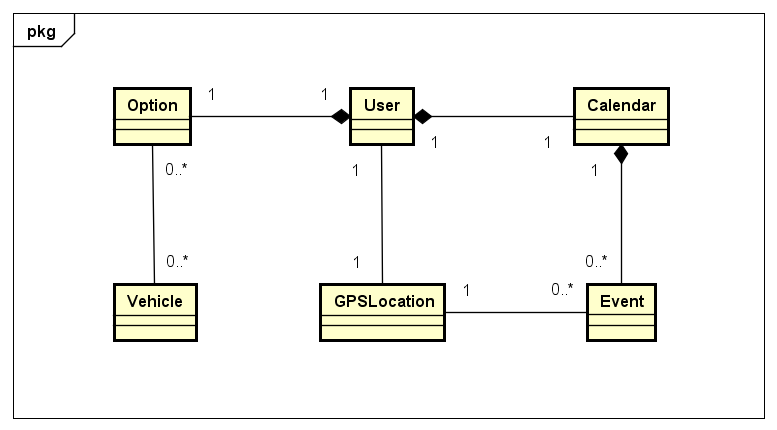
\includegraphics[width=\textwidth]{Img/ClassDiagram0}
	\caption{Class Diagram}
	\label{fig:ClassDiagram0}
\end{sidewaysfigure}
\subsubsection*{Difference between Machine and World}
The following is a distinction between the \textbf{Machine} and the \textbf{World}.
\begin{enumerate}
\item Machine: the Machine is the \textit{Product-to-be} (often also referred to as \textit{System} for short).
\\The \textit{Machine Domain} on the other hand is everything that the Machine can operate onto, meaning that it can manipulate it or more in general it can control.
\item World: the World is the physical world that interacts with the Machine or that it can be observed by it, it's the environment in which the System will gather information and will be affected by the actions performed.
\end{enumerate}
Machine and World are connected by \textit{Shared Phenomena}, the set of events of the World that are observable by the Machine and the ones the Machine can directly cause with its actions.
\\An example of a Shared Phenomena may be something as mundane as the rain, since it's clearly an event that happens in the World and at the same time is observable by the Machine via a forecast or a weather report.
\clearpage
\subsection{Product Functions}
The system allows each user to create their personal calendar by specifying place and time of each appointment and then view the proposed solution, to be more specific the user can:
\begin{enumerate}
\item Register to the system with username and password.
\item Logging to the service.
\item Manage the information of an account and delete it.
\item Specify means of travel preferences.
\item Create an appointment in the calendar.
\item Change appointment information.
\item Delete an appointment.
\item Schedule flexible lunch/breaks of specific length in a given interval.
\end{enumerate}
\par
\subsection{User Characteristics}
The users interested in using the system should be at least familiar with the concept of navigating a web page and using a smartphone in the day to day routine without needing any technical competence regarding the topic, they must be aware of the laws regarding the public circulation on the streets of the country they wish to use the services provided and need a valid driver licence if they want to use a car and they must possess an electronic payment method to use third party car/bike sharing options.
\par
\subsection{Domain Assumptions}
We assume that the following statements are true:
\begin{enumerate}
\item It exists a combination of means of transportation that will take the user to his/her destination even if not before the desired time.
\item The GPS location of the user is always correct.
\item Weather forecasts have a 100\% accuracy.
\item Public transportations always arrive on time.
\item Internet connection is never lost.
\item Is possible to integrate the system with already existing application from third party companies and public transportations.
\end{enumerate}
%Specific Requirements------------------------------------------------
\clearpage
{\color{Blue}{\section{Specific Requirements}}}
\label{sect:Specific Requirements}
\subsection{External Interface Requirements}
\subsubsection{User Interfaces}
The main way the users can interact with the system is via the mobile application for their smartphone, the interface should be user-friendly and in particular easy to read, with large and high contrast text to minimize reading problems in direct sunlight; the second way of connecting to the services provided is to use the web application their personal computer.
In both cases the user interfaces must satisfy the following constrains:
\begin{itemize}
	\item The first page must always ask the user to login or register to service.
	\item After the login, the system redirects the user to his/her home page.
	\item (Web) A toolbar must be present in every page, except login and registration page.
	\item (Mobile) A toolbar must be present in the homepage.
	\item The \emph{Create a meeting} page must provide a guided process to set-up a meeting and clearly show if the created meeting is not reachable in time from the location of a previous appointment.
	\item The \emph{Manage meetings} page must show a list of user's meetings divided by day and hour, and allows the user to select a meeting to obtain further information.
	\item The interface must offer the possibility to choose between a set of different languages.
	\item The user interface must dynamically adapt to the screen size.
	\item The Mobile and Web application must use the same graphical elements.
\end{itemize}
In addition to these constraints, other platform-dependent constraints are provided:
\begin{itemize}
	\item Web Application:\par
		All the pages must submit to W3C standards.
	\item Mobile Application:\par
		All mobile versions must follow the design guidelines provided by the respective platform manufacturer (Android, iOS, Windows \dots).
\end{itemize}
\subsubsection{Hardware Interfaces}
The web application needs any personal computer connected to the internet, while the mobile application must be able to connect to the network in order to exchange information with the server, such as destination and location of the user retrieved via the GPS of the mobile device.\\
Hardware requirements for both are later specified in \autoref{sec:HardwareLimitations}
\clearpage
\subsubsection{Software Interfaces}
\label{sec:SoftwareInterfaces}
Supported browsers for the web application should include Google Chrome, Mozilla Firefox, Opera, Safari, Internet Explorer and Edge, while the mobile application must be available on Android, iOS, Windows Phone and Blackberry OS.\\
The server side of the application requires: 
\begin{itemize}
	\item \href{http://www.oracle.com/technetwork/java/javaee/overview/index.html}{Java EE}, to write the server application that perform the travel computation and the database access.
	\item \href{https://dev.mysql.com/}{MySQL}, to memorize user information and meetings inside a relational database.
\end{itemize}
The client side of the application requires the latest version of the platform SDK.
\subsubsection{Communication Interfaces}
The client communicates to the server via HTTPS protocol using TCP.\\
In addition, the system must be able to use the API of other application in order to retrieves weather and news about road conditions or strike.

\clearpage

\subsection{Functional Requirements}
\subsubsection{Registration}
\paragraph*{Purpose\\}
The main purpose of the \emph{Registration} use case is to provide the user a service which permits the subscription to the system. The user must fill a registration form with his/her personal information and accept the Terms and Conditions of use. After that a confirmation e-mail is sent to the specified e-mail.
\paragraph{Functional Requirements}
\begin{enumerate}[label=R.\arabic*:]
	\item The system must not accept an already registered e-mail.
	\item The user must provide the following information:
	\begin{itemize}
		\item name
		\item surname
		\item e-mail
		\item password
	\end{itemize}
	\item The system cannot allow the user to proceed in the registration process if he/she does not accept the Terms and Conditions of use.
	\item The system must send an e-mail to the user after he/she submits the form.	
	\item The system must generate a unique link for the registration e-mail.
	\item The user must be able to exit the form any time.
\end{enumerate}

\paragraph*{Use Case\\}
The \emph{Registration} use case is analysed in \autoref{tab:registrationTAB}
\paragraph*{Activity Diagram\\}
The activity diagram of the \emph{Registration} use case in showed in \autoref{fig:registrationac}
\paragraph*{Sequence Diagram\\}
The sequence diagram of the \emph{Registration} use case in showed in \autoref{fig:registrationsq}
\newpage
\begin{longtable}{p{0.25\linewidth}|p{0.75\linewidth}}
	\hline
		\label{tab:registrationTAB}
	\textbf{Name} & \textbf{Registration} \\
	\hline
	\textbf{Actors} & Non registered User \\
	\hline
	\textbf{Entry conditions} & \_ \\
	\hline
	\textbf{Flow of events} & 
	\begin{enumerate}
		\item The user asks to the system to register to its service.
		\item The system shows the appropriate form to fill.
		\item The user fills the form inserting its own information.
		\item The user submits the form.
		\item The system checks if the e-mail is unique.
		\item The system sends to the specified e-mail address a confirmation e-mail with a unique link.
		\item The user must open the e-mail and click on the confirmation link.
		\item The system receives the confirmation, saves the data inside a database and notifies to the user.
	\end{enumerate}\\
	\hline
	\textbf{Exit conditions} & The user is now registered and he/she can login and start to use the service.\\
	\hline
	\textbf{Exceptions} & Exceptions can occur when requirements R.1, R.2 and R.3 are violated, in this case the system reloads the registration form and goes back to step 2. 
	Registration process is also aborted when the user decides to complete it. \\
	\hline
	\caption{\emph{Registration} use case description}
\end{longtable}

\begin{figure}[h]
	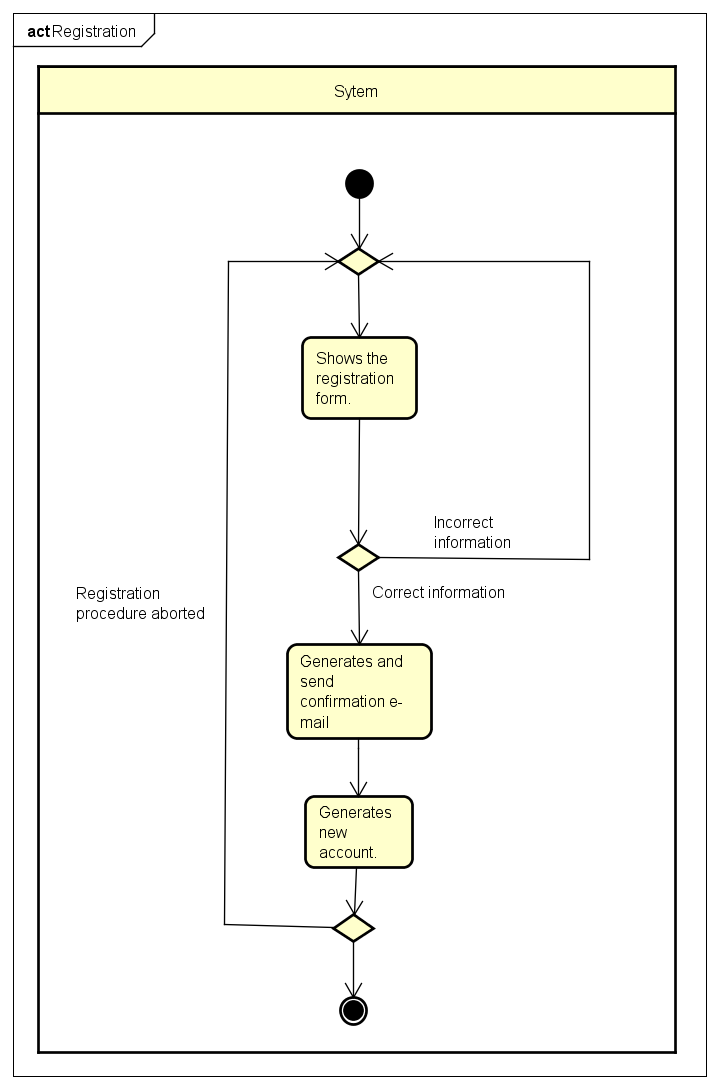
\includegraphics[width=\textwidth, height=\textheight, keepaspectratio=true]{Img/RegistrationAC}
	\caption{\emph{Registration} activity diagram}
	\label{fig:registrationac}
\end{figure}

\begin{figure}
	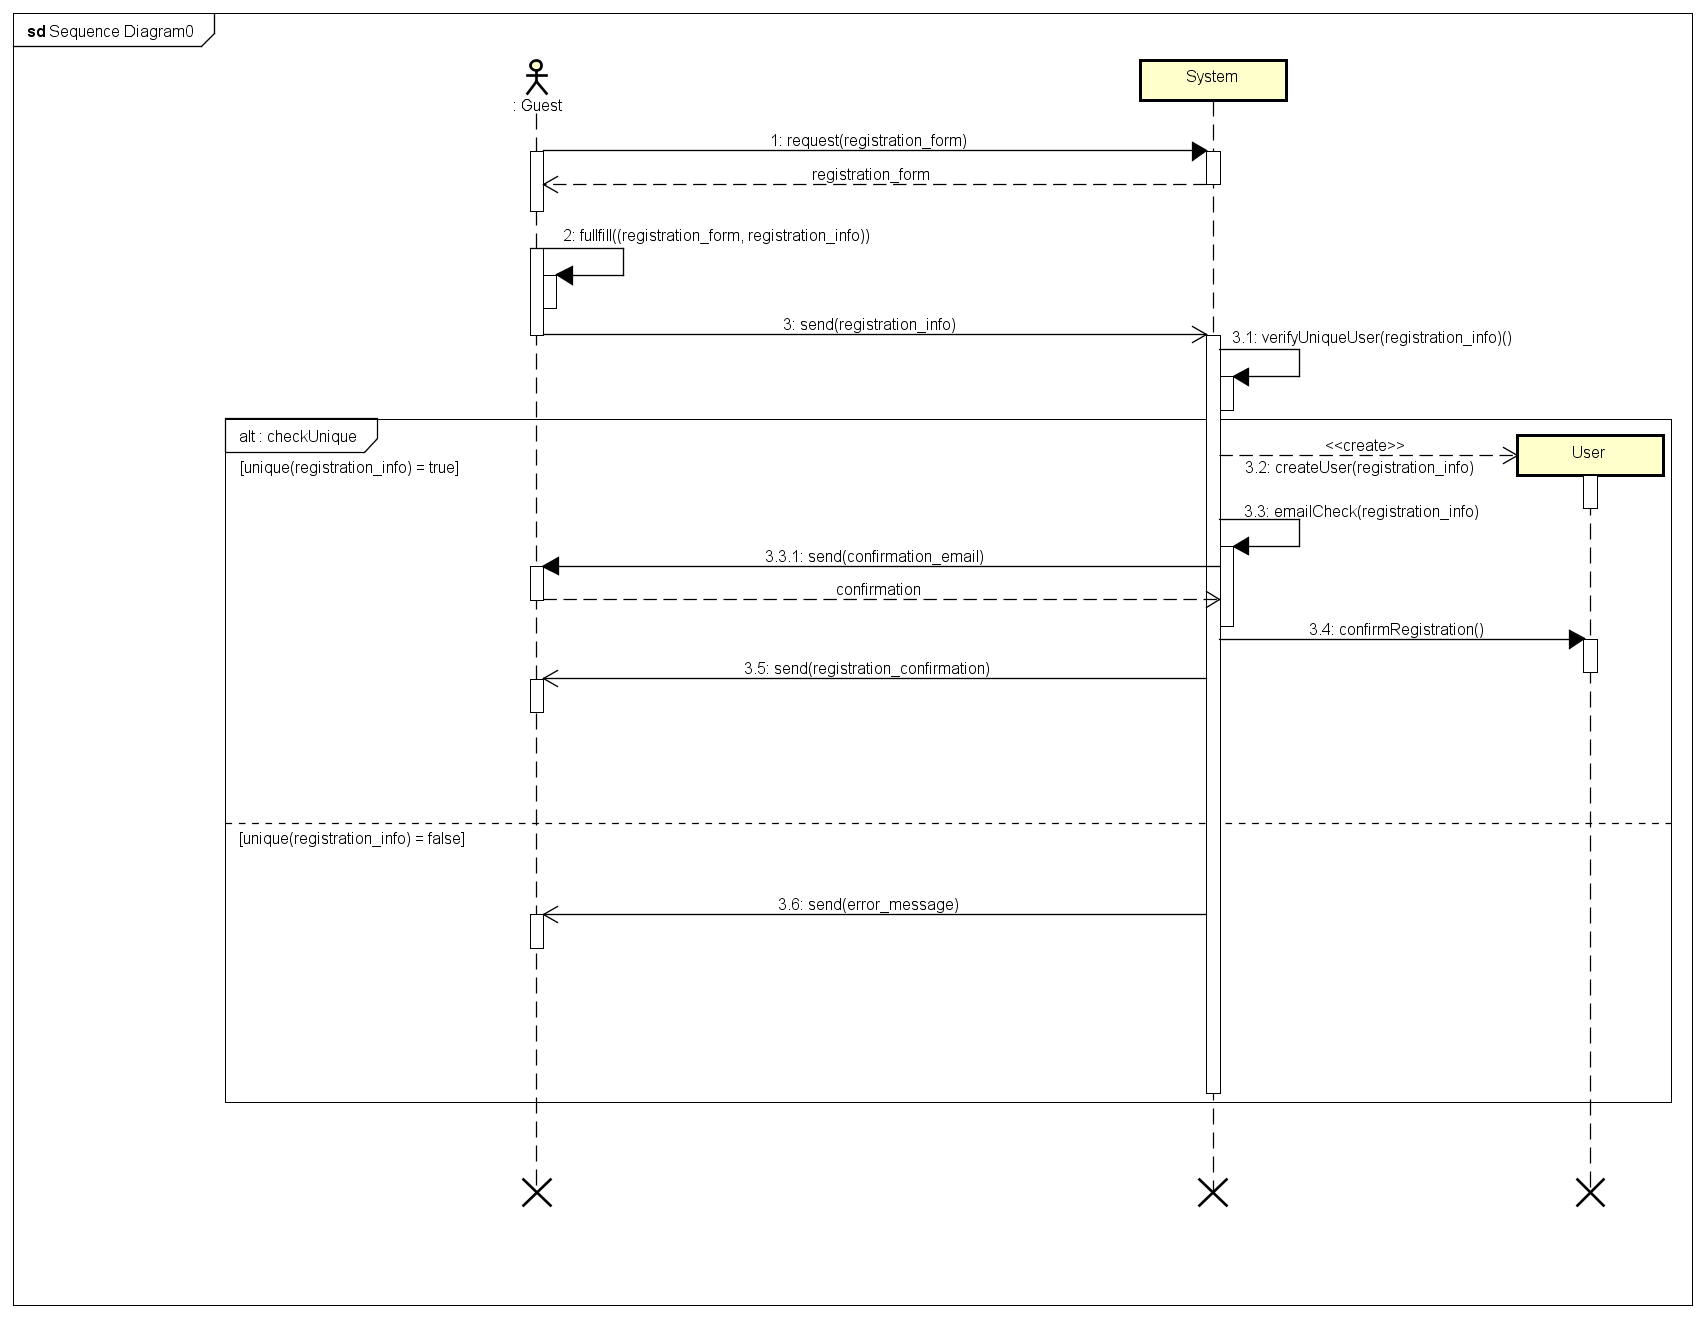
\includegraphics[width=\textheight, height=\textwidth, angle=90, keepaspectratio=true]{Img/RegistrationSQ}
	\caption{\emph{Registration} sequence diagram}
	\label{fig:registrationsq}
\end{figure}

\clearpage
\subsubsection{Specify Means of Travel}
\paragraph*{Purpose\\}
The purpose of this functionality is to allow the user to select an order for his/her favourite means of travel and what vehicles he/she owns, the system will then take this data in consideration once it has to calculate a trip plan by giving precedence to the vehicles higher in the hierarchy.
Both preferred and owned vehicles are optional information, if the user doesn't insert them the system will simply not be influenced when computing travels.

\paragraph*{Functional Requirements}
\begin{enumerate}[label=R.\arabic*:,resume]
	\item The user must be logged in.
	\item A vehicle already selected in an option must not appear again in the list when the user is selecting one.
	\item The user must be able to change the inserted data at any time.
	\item The system must take the preferences into account each time it computes a travel.
\end{enumerate}

\paragraph*{Scenario\\}
Bill loves to move using his bicycle, and wishes to use it each time he can, so he decides to place it as his favourite vehicle by opening the Travlendar + app and after logging in he selects the "Options" icon, then he proceeds to open the "Select favourite vehicles" section and presses the “+” sign to add one, he then chooses "Bicycle" from the list he is presented with.\\
Bill then remembers to also add the Bicycle to his owned vehicles, so the app won't suggest him to use a bike sharing company, to do that he selects the "Owned vehicles" option and just like before he presses the “+” sign and then picks "Bicycle" from the list to add it.

\paragraph*{Use Case\\}
The \emph{Specify Means of Travel} use case is analysed in \autoref{tab:SpecifyMeansofTravelTAB} and in \autoref{fig:SpecifyMeansofTravelUC}
\paragraph*{Activity Diagram\\}
The activity diagram of the \emph{Specify Means of Travel} use case in showed in \autoref{fig:SpecifyMeansofTravelAC}
\paragraph*{Sequence Diagram\\}
The sequence diagram of the \emph{Specify Means of Travel} use case in showed in \autoref{fig:SpecifyMeansofTravelSQ}
\newpage
\begin{longtable}{p{0.25\linewidth}|p{0.75\linewidth}}
	\hline
		\label{tab:SpecifyMeansofTravelTAB}
	\textbf{Name} & \textbf{Specify Means of Travel} \\
	\hline
	\textbf{Actors} & User \\
	\hline
	\textbf{Entry conditions} & The user must be logged in\\
	\hline
	\textbf{Flow of events} & 
	\begin{enumerate}
		\item The user opens the app's options.
		\item The user selects either the option to order the vehicles preferences or the one to add an owned one.
		\item The user selects the “+” sign to add a vehicle.
		\item The system provides a list of vehicles not already selected to the user.
		\item The user chooses a vehicle from the list.
		\item The system stores the choice in the database.
	\end{enumerate}\\
	\hline
	\textbf{Exit conditions} & The user has selected one or more vehicles in his/her preference and/or in the owned section.\\
	\hline
	\textbf{Exceptions} & If the use already selected all possible vehicles the system won’t allow another insertion. \\
	\hline
	\caption{\emph{Specify Means of Travel} use case description}
\end{longtable}

\begin{figure}[h]
	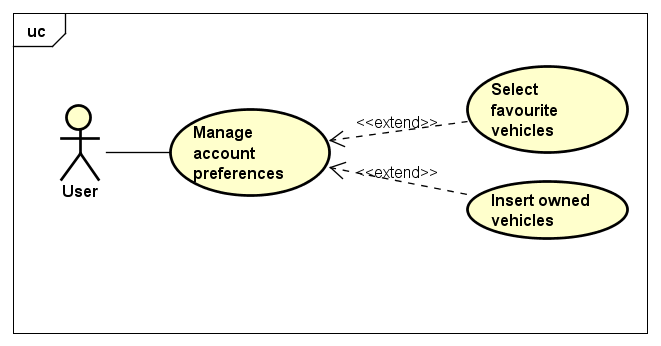
\includegraphics[width=\textwidth]{Img/SpecifyMeansofTravelUC}
	\caption{\emph{Specify Means of Travel} use case}
	\label{fig:SpecifyMeansofTravelUC}
\end{figure}

\begin{figure}[h]
	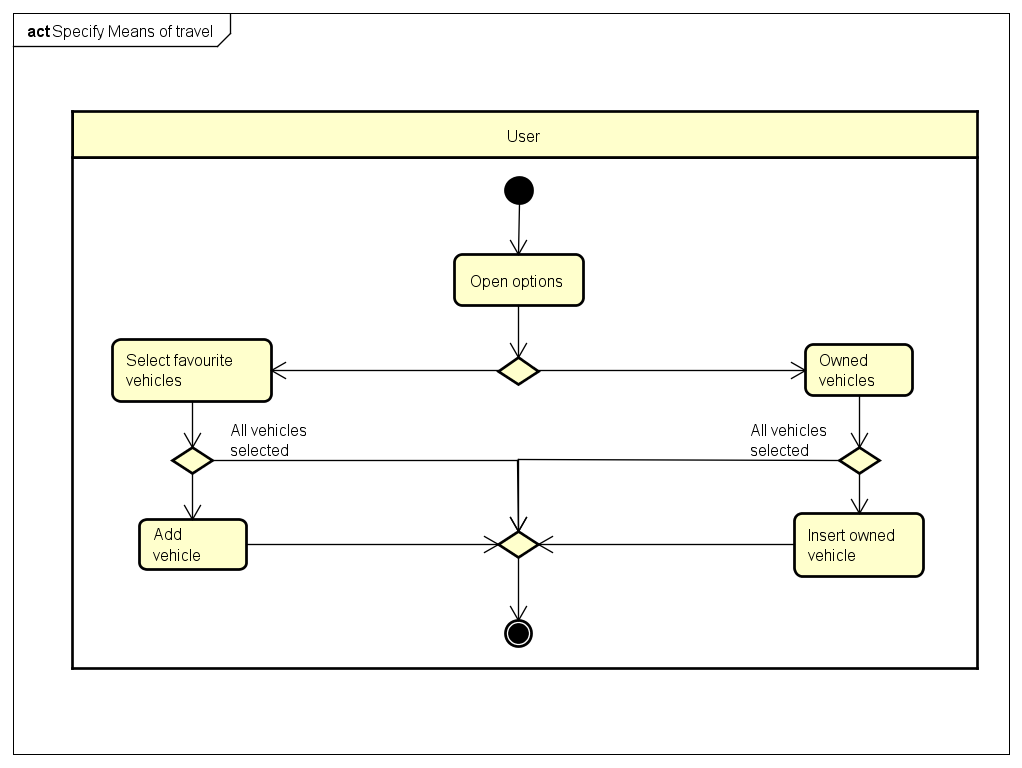
\includegraphics[width=\textheight, height=\textwidth, angle=90, keepaspectratio=true]{Img/SpecifyMeansofTravelAC}
	\caption{\emph{Specify Means of Travel} activity diagram}
	\label{fig:SpecifyMeansofTravelAC}
\end{figure}

\begin{figure}
	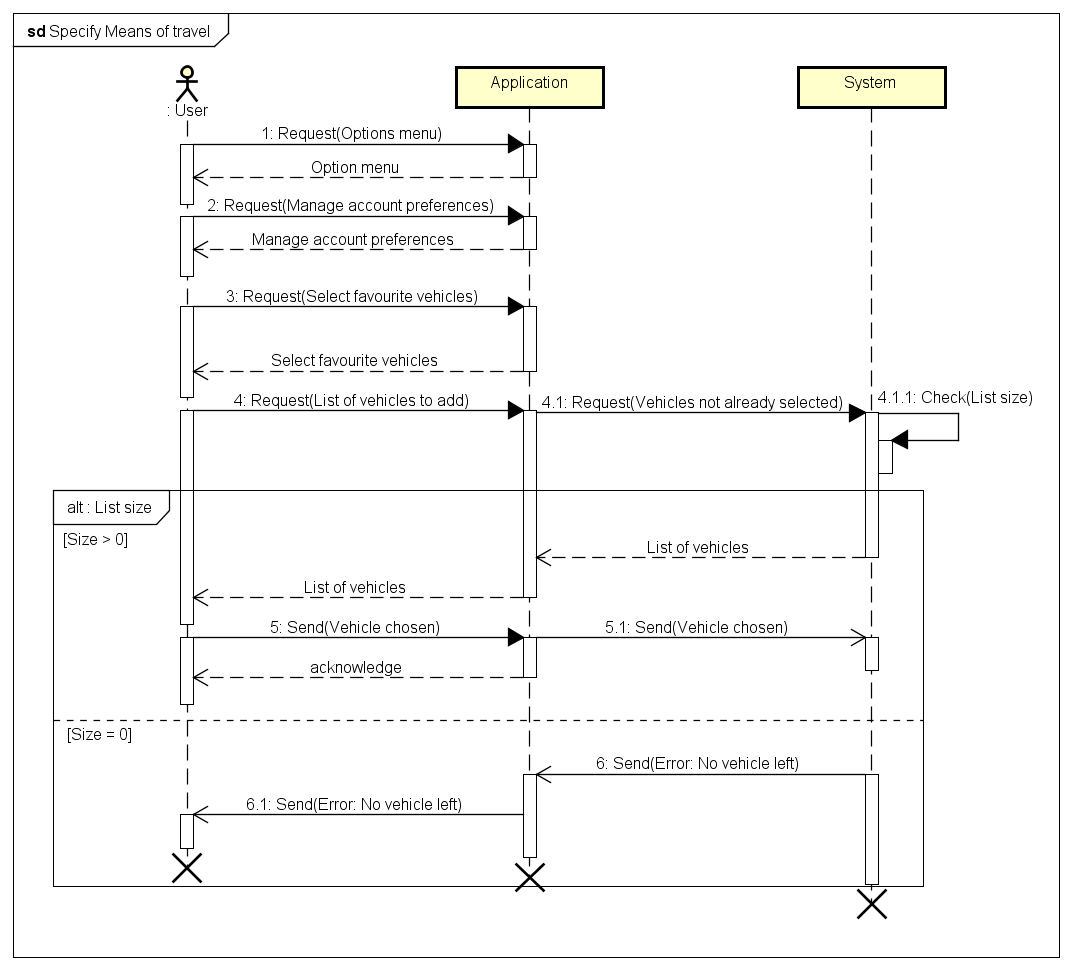
\includegraphics[width=\textheight, height=\textwidth, angle=90, keepaspectratio=true]{Img/SpecifyMeansofTravelSQ}
	\caption{\emph{Specify Means of Travel} sequence diagram}
	\label{fig:SpecifyMeansofTravelSQ}
\end{figure}

\clearpage
\subsubsection{Change Appointment Information}
\label{ChangeAppointmentInformation}
\paragraph*{Purpose\\}
This function allows the user to select an appointment already registered in the calendar and then change parameters ash he/she wishes, the system will then compute again the trip and store the changes made in the database.
\paragraph*{Functional Requirements}
\begin{enumerate}[label=R.\arabic*:,resume]
	\item The user must be logged in.
	\item The user must have at least one upcoming event saved.
	\item The user must be able to change information as many times as he/she wishes.
	\item Past events cannot be changed.
\end{enumerate}

\paragraph*{Scenario\\}
Anna has taken an appointment with her doctor for next week at 3:00 pm and she already recorded it using Travlendar+, but she remembers that she has to bring her son to football practice before 3:15 pm, she decides then to call her doctor and re-schedules the appointment for 2:00 pm, once the call is finished she opens Travlendar+ and proceeds to open "Manage meetings", and then after selecting the appointment selects "Change meeting details", where she can change the time of the appointment and then saves it.
\paragraph*{Use Case\\}
The \emph{Change Appointment Information} use case is analysed in \autoref{tab:ChangeAppointmentInformationTAB} and in \autoref{fig:ChangeAppointmentInformationUC}
\paragraph*{Activity Diagram\\}
The activity diagram of the \emph{Change Appointment Information} use case in showed in \autoref{fig:ManageAppointmentsAC}
\paragraph*{Sequence Diagram\\}
The sequence diagram of the \emph{Change Appointment Information} use case in showed in \autoref{fig:ChangeAppointmentInformationSQ}
\newpage
\begin{longtable}{p{0.25\linewidth}|p{0.75\linewidth}}
	\hline
		\label{tab:ChangeAppointmentInformationTAB}
	\textbf{Name} & \textbf{Change Appointment Information} \\
	\hline
	\textbf{Actors} & User \\
	\hline
	\textbf{Entry conditions} & The user must be logged in and must have at least one upcoming event.\\
	\hline
	\textbf{Flow of events} & 
	\begin{enumerate}
		\item The user opens the app.
		\item The user selects the "Manage meetings" section.
		\item The user selects the meeting he/she wants to change.
		\item The user selects "Change meeting details".
		\item The user changes the meeting as he/she wishes by providing at least one of the following:
	\begin{enumerate}
	\item Date of the meeting.
	\item Time of the meeting.
	\item Location of the meeting.
	\item Name of the meeting.
	\end{enumerate}
		\item The user saves the changes.
		\item The system updates the meeting in the database and computes again the trip.
	\end{enumerate}\\
	\hline
	\textbf{Exit conditions} & The user changed a meeting.\\
	\hline
	\textbf{Exceptions} & If the meeting has expired and the user tries to change it, the application will avoid it. \\
	\hline
	\caption{\emph{Change Appointment Information} use case description}
\end{longtable}

\begin{figure}[h]
	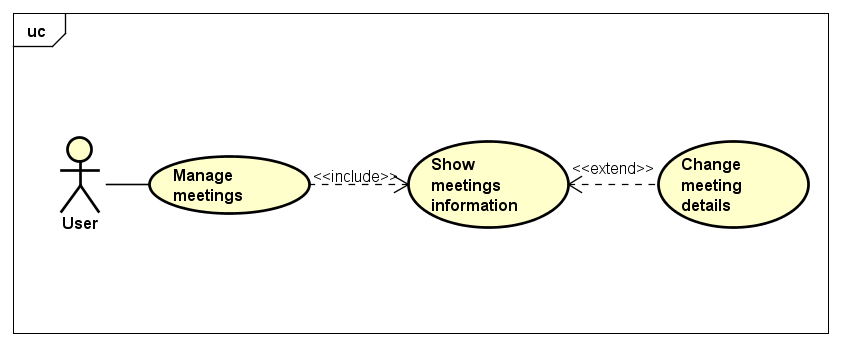
\includegraphics[width=\textwidth]{Img/ChangeAppointmentInformationUC}
	\caption{\emph{Change Appointment Information} use case}
	\label{fig:ChangeAppointmentInformationUC}
\end{figure}

\begin{figure}[h]
\centering
	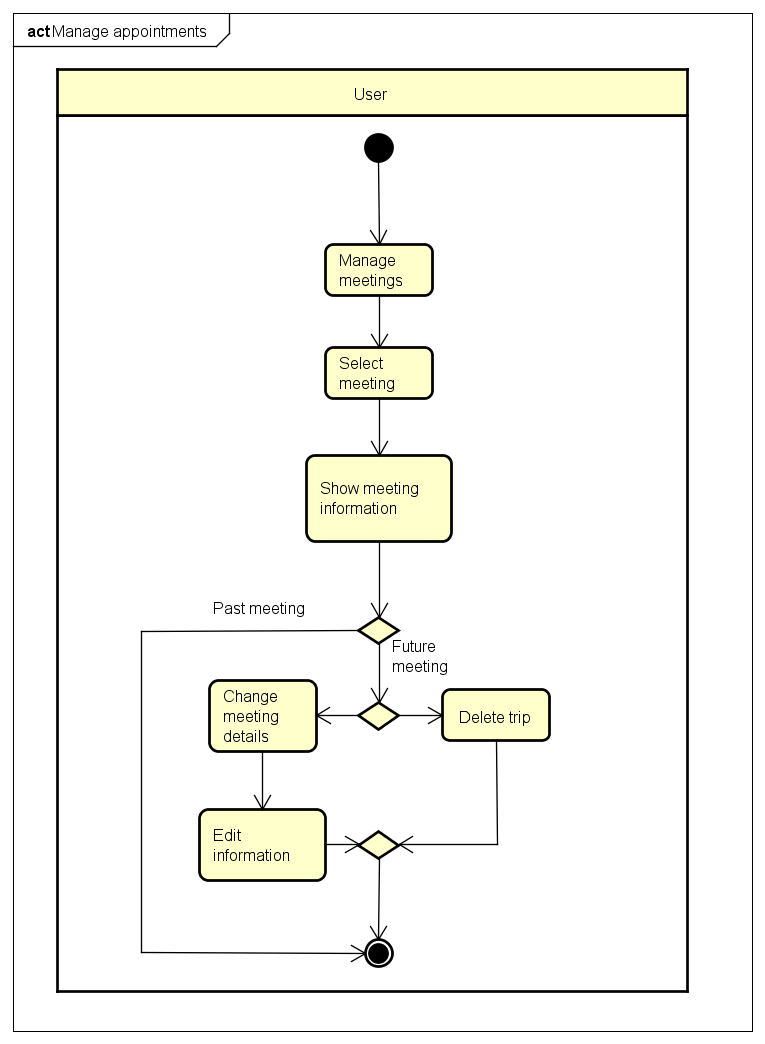
\includegraphics[width=\textheight, height=\textwidth, keepaspectratio=true]{Img/ManageAppointmentsAC}
	\caption{\emph{Change Appointment Information \& Delete Appointment} activity diagram}
	\label{fig:ManageAppointmentsAC}
\end{figure}

\begin{sidewaysfigure}
	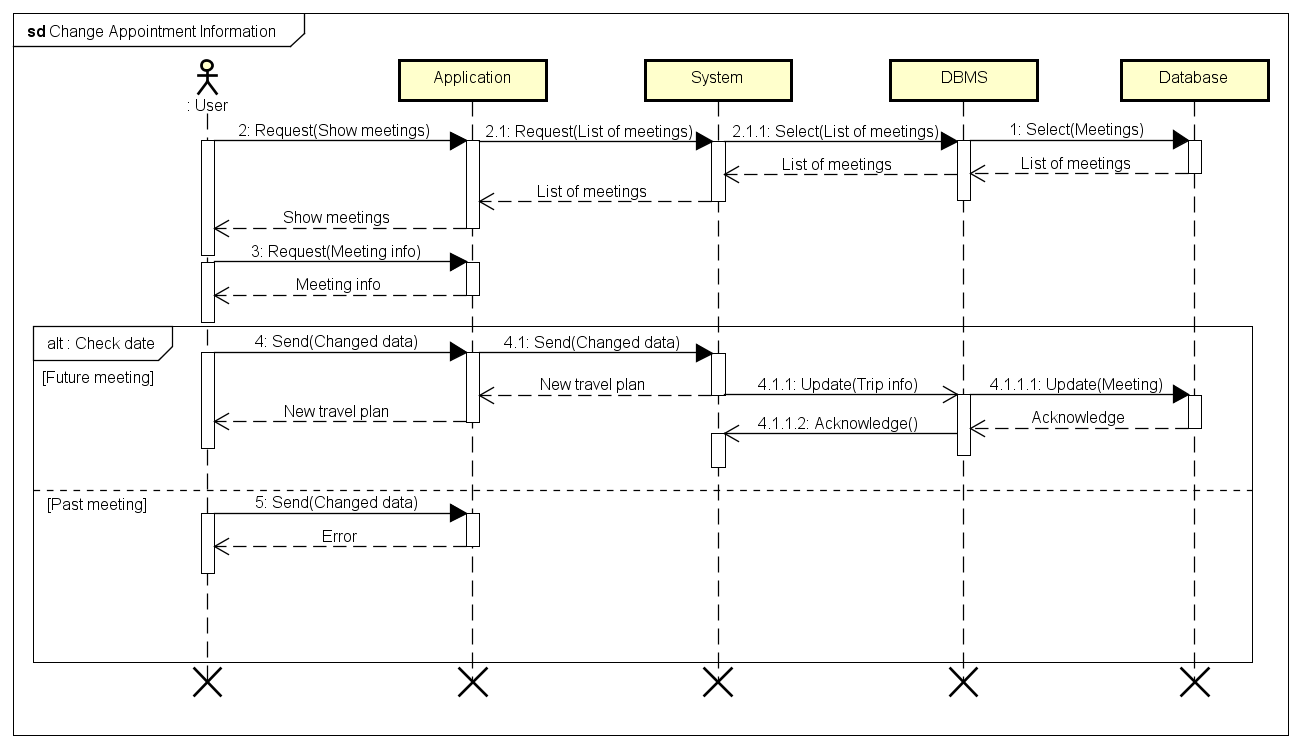
\includegraphics[width=\textheight, height=\textwidth, keepaspectratio=true]{Img/ChangeAppointmentInformationSQ}
	\caption{\emph{Change Appointment Information} sequence diagram}
	\label{fig:ChangeAppointmentInformationSQ}
\end{sidewaysfigure}

\clearpage
\subsubsection{Delete Appointment}
\paragraph*{Purpose\\}
\paragraph*{Functional Requirements}
\begin{enumerate}[label=R.\arabic*:,resume]
	\item The user must be logged in.
	\item The user must have at least one upcoming event saved.
	\item Once a meeting is deleted all data regarding it is lost.
	\item Past events cannot be deleted.
\end{enumerate}

\paragraph*{Scenario\\}
Emily decided with her friends to go out for dinner Saturday and inserted the place and time in a meeting using Travlendar+, but one of the other girls later proposed to have dinner at home, and since Emily has the biggest dining room she invited all the others to her place, since she doesn't need any more a travel planned she deletes the meeting previously created by selecting it in the "Manage meetings" section, she then proceeds to remove it by pressing the "Delete trip" button.
\paragraph*{Use Case\\}
The \emph{Delete Appointment} use case is analysed in \autoref{tab:DeleteAppointmentTAB} and in \autoref{fig:DeleteAppointmentUC}
\paragraph*{Activity Diagram\\}
The activity diagram of the \emph{Delete Appointment} use case in showed in \autoref{fig:ManageAppointmentsAC} alongside \emph{Change Appointment Information} from \autoref{ChangeAppointmentInformation}.
\paragraph*{Sequence Diagram\\}
The sequence diagram of the \emph{Delete Appointment} use case in showed in \autoref{fig:DeleteAppointmentSQ}
\newpage
\begin{longtable}{p{0.25\linewidth}|p{0.75\linewidth}}
	\hline
		\label{tab:DeleteAppointmentTAB}
	\textbf{Name} & \textbf{Delete Appointment} \\
	\hline
	\textbf{Actors} & User \\
	\hline
	\textbf{Entry conditions} & The user must be logged in and must have at least one upcoming event.\\
	\hline
	\textbf{Flow of events} & 
	\begin{enumerate}
		\item The user opens the app.
		\item The user selects the "Manage meetings" section.
		\item The user selects the meeting he/she wants to delete.
		\item The user presses the "Delete trip" button.
		\item The system sends the delete request to the DBMS.
		\item The DBMS deletes the entry selected by the user from the database.
	\end{enumerate}\\
	\hline
	\textbf{Exit conditions} & A meeting was deleted.\\
	\hline
	\textbf{Exceptions} & If the meeting has expired and the user tries to delete it, the application will avoid it. \\
	\hline
	\caption{\emph{Delete Appointment} use case description}
\end{longtable}

\begin{figure}[h]
	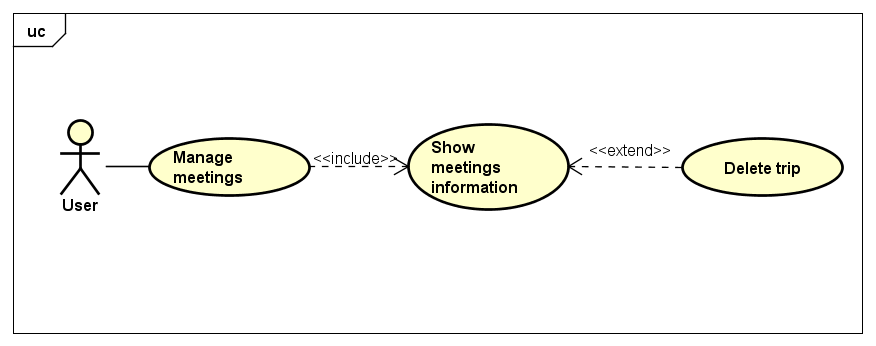
\includegraphics[width=\textwidth]{Img/DeleteAppointmentUC}
	\caption{\emph{Delete Appointment} use case}
	\label{fig:DeleteAppointmentUC}
\end{figure}

\begin{sidewaysfigure}
	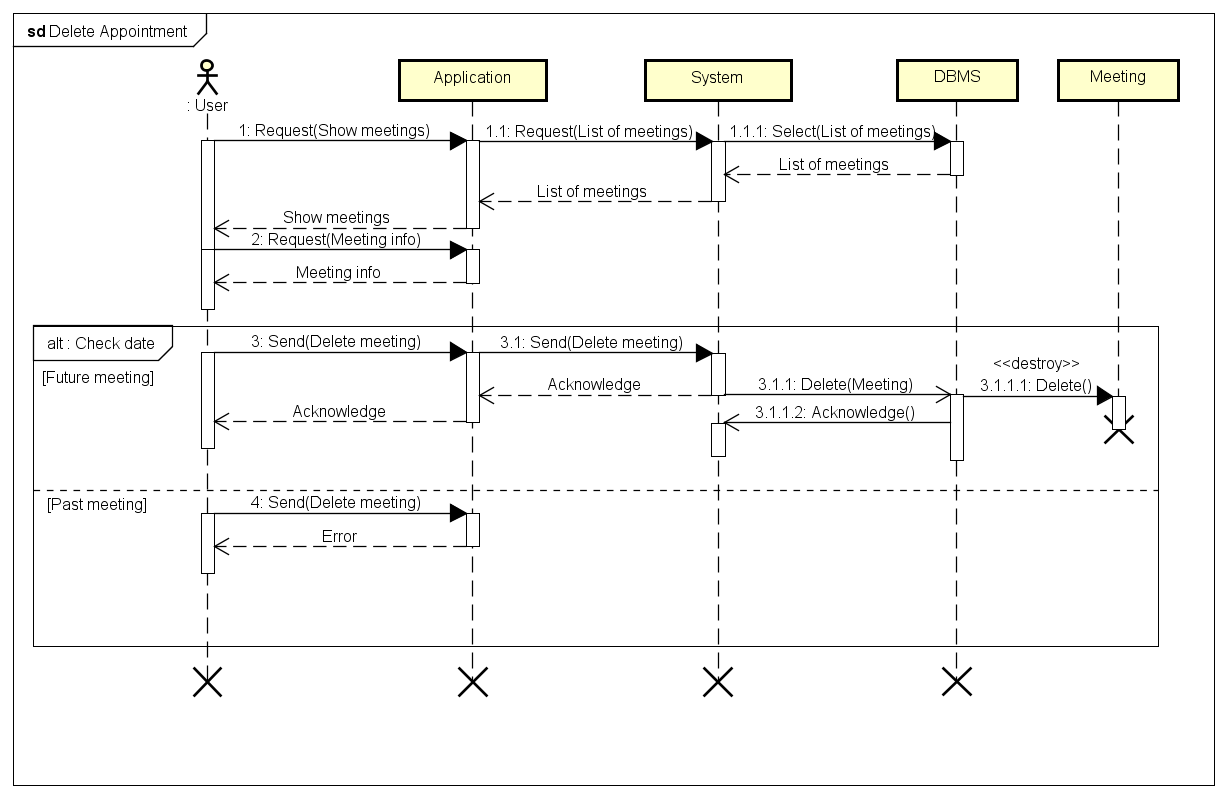
\includegraphics[width=\textheight, height=\textwidth, keepaspectratio=true]{Img/DeleteAppointmentSQ}
	\caption{\emph{Delete Appointment} sequence diagram}
	\label{fig:DeleteAppointmentSQ}
\end{sidewaysfigure}

\clearpage
\subsubsection{Manage Breaks}
\paragraph*{Purpose\\}
The functionality delivered by \emph{Manage Breaks} refers to the possibility of scheduling a flexible time in which the system will reserve a given amount of minutes to any kind of break, with the option of changing or deleting said break in the future.\\
\textbf{Note} that we will focus on the creating aspect, since treating also changing and deleting would offer no additional insight.
\paragraph*{Functional Requirements}
\begin{enumerate}[label=R.\arabic*:,resume]
	\item The user must be logged in.
	\item The user must insert the following parameters:
	\begin{enumerate}
	\item Starting time (From).
	\item Duration of the break.
	\item Days of the week.
	\item End time (To).
	\end{enumerate}
\end{enumerate}
\paragraph*{Scenario\\}
Jimmy has a 3 hours window on Monday between school and soccer practice, from 12:30 am to 15:30 am in which he wants to have lunch and then study the remaining time.\\
He decides to use Travlendar+ to schedule a flexible break, first he opens the app on his smartphone, then after going into "Manage account preferences" he adds a break of 30 minutes in the spare time he has by using the "Create break" option and filling the necessary fields.
\paragraph*{Use Case\\}
The \emph{Create Breaks} use case is analysed in \autoref{tab:CreateBreaksTAB}, in \autoref{fig:ManageBreaksUC} are also represented the "Delete break" and "Change break" functions.
\paragraph*{Activity Diagram\\}
The activity diagram of the \emph{Manage Breaks} use case in showed in \autoref{fig:ManageBreaksAC}
\paragraph*{Sequence Diagram\\}
The sequence diagram of the \emph{Create Breaks} use case in showed in \autoref{fig:CreateBreaksSQ}
\newpage
\begin{longtable}{p{0.25\linewidth}|p{0.75\linewidth}}
	\hline
		\label{tab:CreateBreaksTAB}
	\textbf{Name} & \textbf{Create Breaks} \\
	\hline
	\textbf{Actors} & User \\
	\hline
	\textbf{Entry conditions} & The user must be logged in.\\
	\hline
	\textbf{Flow of events} & 
	\begin{enumerate}
		\item The user opens the app.
		\item The user opens the options menu.
		\item The user enters in "Manage account preferences".
		\item The user selects "Create break".
		\item The user fills the requested fields with the desired information.
		\item The user saves the changes.
		\item The system sends the data to the DBMS.
		\item The DBMS stores the data about the break.
	\end{enumerate}\\
	\hline
	\textbf{Exit conditions} & The user created a break\\
	\hline
	\textbf{Exceptions} & If the user doesn't choose a day of the week the system will act like if every day was selected. \\
	\hline
	\caption{\emph{Create Breaks} use case description}
\end{longtable}

\begin{figure}[h]
	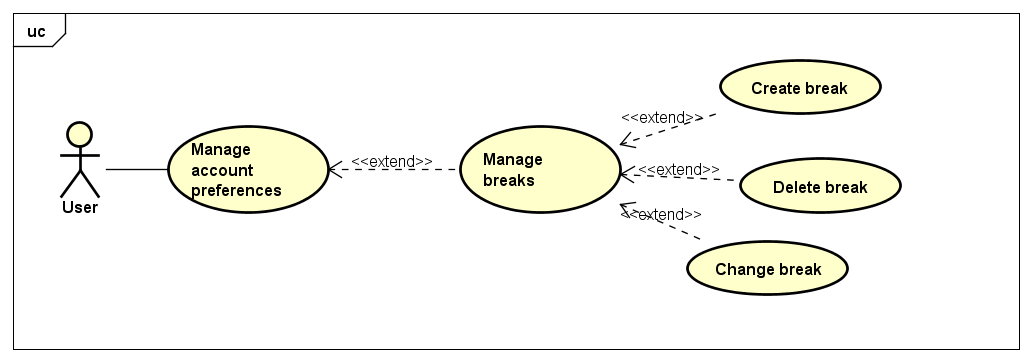
\includegraphics[width=\textwidth]{Img/ManageBreaksUC}
	\caption{\emph{Create Breaks} use case}
	\label{fig:ManageBreaksUC}
\end{figure}

\begin{figure}[h]
\centering
	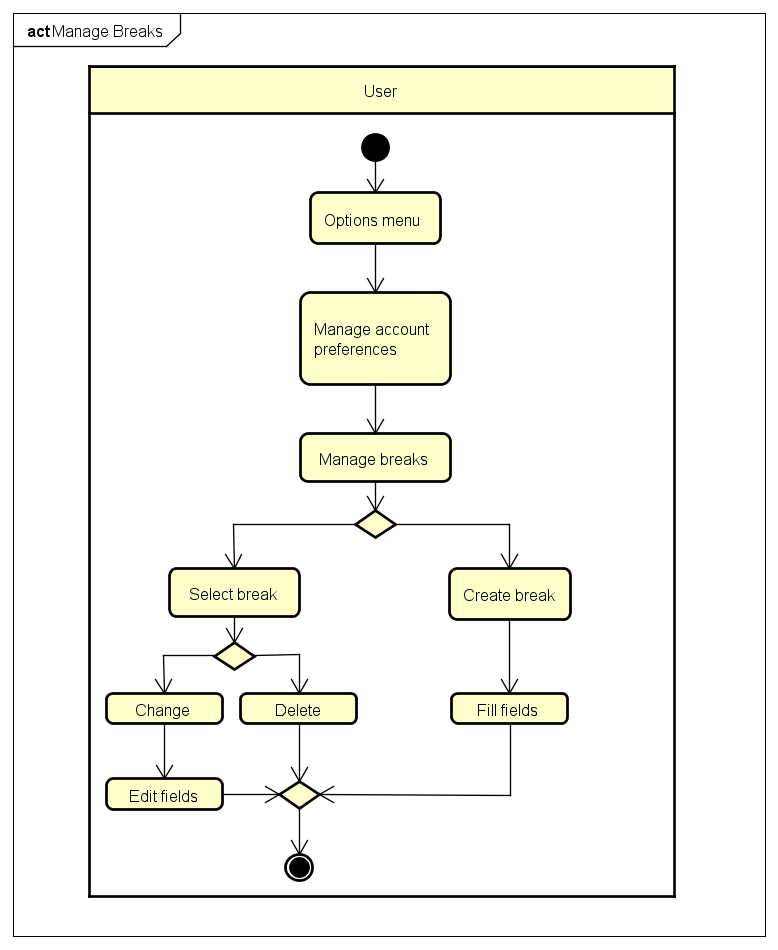
\includegraphics[width=\textheight, height=\textwidth, keepaspectratio=true]{Img/ManageBreaksAC}
	\caption{\emph{Manage Breaks} activity diagram}
	\label{fig:ManageBreaksAC}
\end{figure}

\begin{sidewaysfigure}
	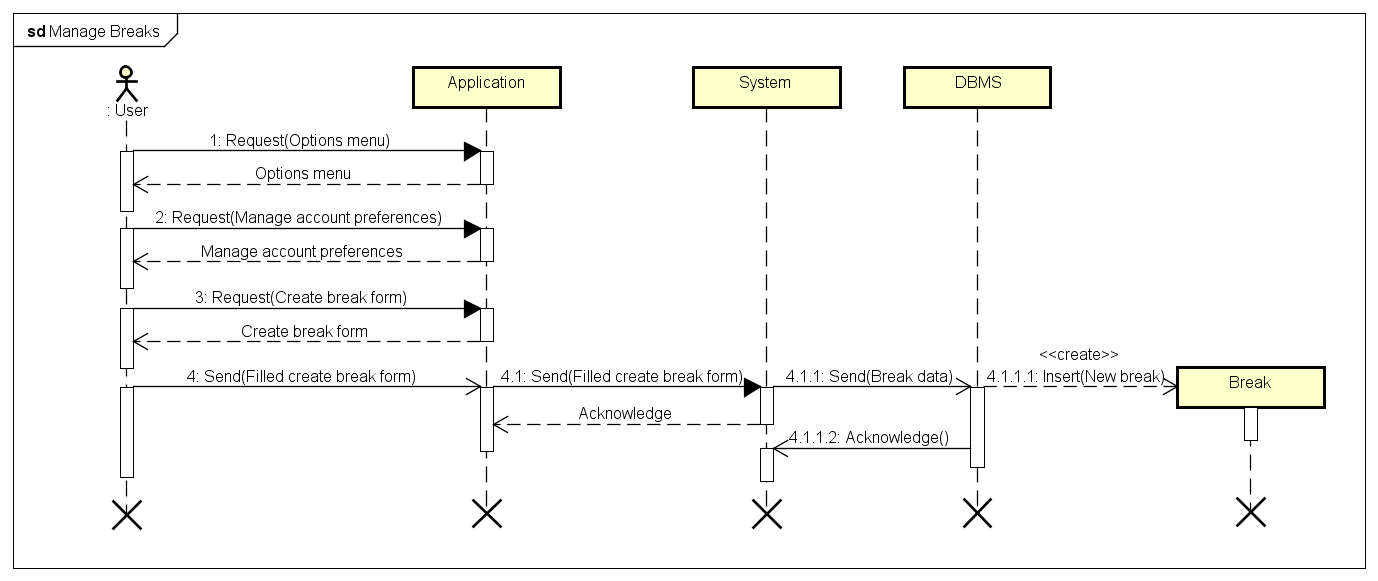
\includegraphics[width=\textheight, height=\textwidth, keepaspectratio=true]{Img/CreateBreaksSQ}
	\caption{\emph{Create Breaks} sequence diagram}
	\label{fig:CreateBreaksSQ}
\end{sidewaysfigure}
%Add Use cases----------------------------------------------------
\clearpage
\subsection{Performance Requirements}
Without taking into consideration the speed of the internet connection, in order to guarantee an acceptable user experience the following  requirements must be satisfied:
\begin{itemize}
\item Navigation between pages of the system must happen in 0.5s or less.
\item The  best travel plan must be computed in 5s or less.
\item No limit of registered users in the database.
\item No limit of schedulable appointments.
\item At least 1000 users must be able to use the service at the same time. 
\end{itemize}
\newpage
\subsection{Design Constraints}
\subsubsection{Standards Compliance}
The web application must comply with the standards dictated by W3C, while the mobile application must follow the Oracle guidelines for Java programming.
\subsubsection{Hardware Limitations}
\label{sec:HardwareLimitations}
Minimum system requirements for the two applications:
\begin{itemize}
\item Web application
\begin{itemize}
\item 512Mb of RAM.
\item 2Mb/s internet connections.
\item 800X600 screen resolution.
\end{itemize}
\item Mobile application
\begin{itemize}
\item 1Gb of RAM.
\item 3G UMTS internet connections.
\item 100Mb of free space.
\end{itemize}
\end{itemize}
The system should also be able to process operations in parallel.
\clearpage
\subsection{Software System Attributes}
\subsubsection{Reliability}
Each trip plan computed given the preferences expressed by the user and the weather forecast and strikes must not differ more than 5\% from the optimal travel distance or ETA.
\subsubsection{Availability}
The system to be must guarantee an availability of no less than 98\%.
\subsubsection{Safety and Privacy Constraints}
The user oversees his/her own security while travelling and must grant access to the current location, information about former trips and personal data are stored but only the user itself has access to them.
\subsubsection{Maintainability}
The system must be developed in such a way that future implementation of new features and changes to existing ones can be done seamlessly, in other words the system has to be modular and scalable.
\subsubsection{Portability}
As already mentioned in \autoref{sec:SoftwareInterfaces} the software must be available on different configurations, it must be as environment independent as possible, meaning that it has to work on different platforms with the minimum amount of changes to the software itself.




\end{document}